\documentclass[journal,peerreview,onecolumn]{IEEEtran}
% \documentclass[journal]{IEEEtran}

\usepackage{cite}
\usepackage[pdftex]{graphicx}
\graphicspath{{./Fig/}}
\DeclareGraphicsExtensions{.pdf,.jpg,.png}
\usepackage{amsmath,amssymb,amsthm}
\usepackage{algorithm}
\usepackage{algorithmic}
\usepackage{array}
\usepackage[caption=false,font=footnotesize]{subfig}
\usepackage{fixltx2e}
\usepackage{url}
\usepackage{listings}
\usepackage{multirow}
\usepackage{tikz}
\usepackage{pgfplots}
\usepackage{tabularx}
\usepackage{empheq}

\newcommand\MyBox[2]{
  \fbox{\lower0.75cm
    \vbox to 1.2cm{\vfil
      \hbox to 1.2cm{\hfil\parbox{1.4cm}{#1\\#2}\hfil}
      \vfil}%
  }%
}

% for peerreview
\usepackage{setspace}
\onehalfspacing

\newtheorem{prop}{Proposition}

% correct bad hyphenation here
% \hyphenation{op-tical net-works semi-conduc-tor}

\begin{document}
%
% paper title
% Titles are generally capitalized except for words such as a, an, and, as,
% at, but, by, for, in, nor, of, on, or, the, to and up, which are usually
% not capitalized unless they are the first or last word of the title.
% Linebreaks \\ can be used within to get better formatting as desired.
% Do not put math or special symbols in the title.
\title{Operational Feature Selection in Gaussian Mixture Models}
%
%
% author names and IEEE memberships
% note positions of commas and nonbreaking spaces ( ~ ) LaTeX will not break
% a structure at a ~ so this keeps an author's name from being broken across
% two lines.
% use \thanks{} to gain access to the first footnote area
% a separate \thanks must be used for each paragraph as LaTeX2e's \thanks
% was not built to handle multiple paragraphs
%

\author{Adrien~Lagrange,~Mathieu~Fauvel~and~Manuel~Grizonnet% <-this % stops a space
\thanks{A. Lagrange and M. Fauvel are with the Université de Toulouse,
INP-ENSAT, UMR 1201 DYNAFOR, France and with the INRA, UMR 1201
DYNAFOR, France.}
\thanks{M. Grizonnet is with Centre Nat. d'Etudes Spatiales, French Space Agency, Toulouse, France.}}

% The paper headers
\markboth{Transactions on Computational Imaging,~Special Issue on Computational Imaging for Earth Sciences, September~2016}{}

% make the title area
\maketitle

% As a general rule, do not put math, special symbols or citations
% in the abstract or keywords.
\begin{abstract}
This article presents a forward feature selection algorithm based on Gaussian mixture model (GMM) classifiers. The algorithm selects iteratively features that maximize a criterion function which can be either a classification rate or a measure of divergence. Several variations of this algorithm are explored by changing the criterion function and also by testing a floating forward variation allowing backward step to discard already selected features.

An important effort is made in exploiting GMM properties to implement a fast algorithm. In particular, update rules of the GMM model are used to compute the criterion function with various sets of features. The result is a C++ remote module for the remote sensing processing toolbox Orfeo (OTB) developed by CNES.

Finally, the method is tested and also compared to other classifiers using two different datasets, one of hyperspectral images with a lot of spectral variables and one with heterogeneous spatial features. The results validate the fact that the method performs well in terms of processing time and classification accuracy in comparison to the standard classifiers available in OTB.\\
\end{abstract}

% Note that keywords are not normally used for peerreview papers.
% \begin{IEEEkeywords}
% remote sensing, hyperspectral imaging, feature selection, gaussian mixture model, fast computing.
% \end{IEEEkeywords}

% For peer review papers, you can put extra information on the cover
% page as needed:
% \ifCLASSOPTIONpeerreview
% \begin{center} \bfseries EDICS Category: 3-BBND \end{center}
% \fi
%
% For peerreview papers, this IEEEtran command inserts a page break and
% creates the second title. It will be ignored for other modes.
\IEEEpeerreviewmaketitle

\section{Introduction}
\label{sec:intro}

\IEEEPARstart{W}{ith} the increasing number of remote sensing missions, the quantity of data available for a given landscape becomes larger and larger. Several missions are about to produce huge amount of data or have already produced it. After 2018, the EnMAP (Environmental Mapping and Analysis Program) satellites missioned by the German space agency will produce images with 244 spectral bands with a resolution of 30x30m and revisit every 4 days\cite{Müller09enmap}. The Hyperspectral Infrared Imager (HyspIRI) of NASA will also take images with 212 spectral bands every 5 days. Additionally to hyperspectral data, hypertemporal data are also developping. The European satellites Sentinel-2 were launched successfully recently and the hypertemporal data produced by this mission will be fully available at the end of 2016\cite{drusch2012sentinel}.

However, processing this data is more and more challenging because of statistical and computational issues. This statistical issues are often referred as the \emph{curse of dimensionality}. The Hughes phenomenon \cite{hughes1968mean} states that with a given number of samples, prediction accuracy will decays when the complexity is higher than some optimum value. The problem is the fast increase of the number of parameters to estimate in order to build a model when dimension expands \cite{bouveyron2014model}. Thus, a important number of labeled samples is needed to perform learning. For example, in the case of Gaussian Mixture Models, the number of parameters progresses quadratically with the dimension, e.g. with 200 describing variables, the model estimation requires at least around 20,000 samples by class.

The computational issues are multiple. The computing infrastructure needed to process data is more and more expensive because the processing might requires a GPU and a large amount of RAM to load images which can weight a dozen of gigabytes \cite{christophe2011remote}\cite{plaza2011high}. The processing time is also limiting and requires to use parallelize computing (GPU, multi-threading).

A possible method to solve these issues is to perform a reduction of dimension. It is possible to extract a set of relevant features to get a parsimonious representation of the data \cite{jimenez1998supervised}.

For instance, in land-cover classification, given a set of spatial, temporal and spectral features, it is possible to extract those which are the most discriminant for the purpose of classification \cite{fassnacht2014comparison}. In hyperspectral data analysis from the hundreds of available spectral channels, it is possible to reduce the number of channels to make the processing more efficient in terms of statistical complexity because of the reduction of the number of parameters to estimate and thus also in term of computational time. Moreover, dimensional reduction might improves the capacity of generalization of the classifier and avoid overfitting.

There are two ways to reduce dimension \cite{Guyon:2006:FEF:1208773}: features extraction and feature selection. Feature extraction means creating new features by combining the existing ones, for example linear combination as in Principal Component Analysis \cite{jimenez1998supervised}. To the contrary, features selection selects a subset of existing features. It has the advantage to be much more interpretable for the end-user. The selected subset of features corresponds to the most important features for the given task.

There is a large diversity of methods for feature selection. However, they usually do not scale well with the number of pixels to be processed \cite{fauvel2015fast}. Nevertheless, methods based on Gaussian Mixture Models (GMM) have several interesting properties that make them suitable for feature selection in the context of large amount of data. By taking advantage of their intrinsic properties, it is possible to increase the computational efficiency with respect to standard implementation.

Several strategy have been explored to perform feature selection and, among them, wrapper methods receive a certain interest of the community. Wrapper methods can be seen as a search method to determine the best subset of variables for a given learning model. As exhaustive searches are out of question in a practical amount of time, numerous search strategies have been designed. Some optimal are under particular hypothesis \cite{narendra1977branch} and other suboptimal but easier to set up \cite{whitney1971direct}\cite{somol1999adaptive}. Such methods have the advantage to tune the selection to make the most of a particular classifier but require the training of multiple models to test various set of variables which can make them slow if the training is not optimized.

This work proposes to develop a forward feature selection method using GMM in continuation of \cite{fauvel2015fast} and an upgraded floating forward method. The basic method selects iteratively the meaningful features. At each step, the pool of selected features is used to train a GMM which allows to compute a criterion function then used to rank features at the next iteration. The upgraded method introduces possible backward steps after each addition of a feature. An efficient implementation of the method is presented in order to handle large amount of data. Moreover, the developed algorithm is made available as a remote module of the C++ Orfeo Toolbox \cite{christophe2008orfeo}. Finally, tests are conducted to compare different variations of the method and to compare also to other classifiers (GMM, Random Forest, k-nearest-neighbor) available in the Orfeo Toolbox.

The remaining of this article is organized as follows. Section~\ref{sec:gmm-hd} presents Gaussian Mixture Model classifiers and the features selection methods used to make them suitable for high-dimension space. The work done to develop a smart implementation of the proposed selection method is presented in Section~\ref{sec:implementation}. And finally, the tests conducted to explore variations of the algorithm and to compare it to other standard classifiers are detailed in Section~\ref{sec:test}.

\section{Gaussian Mixture Models in high dimension space}
\label{sec:gmm-hd}

In the remaining of the paper, the following notations are used. $\mathcal{S} = \{\mathbf{x}_i,y_i\}_{i=1}^{n}$ denotes the training set where $\mathbf{x}_i \in \mathbb{R}^d$ is the vector of features of the $i^{th}$ sample, $y_i = 1,...,C$ the associated label, C the total number of classes, $n$ the number of samples and $n_c$ the number of samples of class $c$.

    \subsection{Gaussian Mixture Models}

    The hypothesis of mixture models is that a given sample is the realization of a random vector which distribution is a mixture (convex combination) of several class conditioned distribution:
    \begin{equation}
        p(\mathbf{x}) = \sum_{c=1}^{C} \pi_c f_c(\mathbf{x}|\theta)
    \end{equation}
    where $\pi_c$ is the prior i.e. the proportion of class $c$ and $f_c$ a probability density function parametrized by $\theta$.

    The Gaussian mixture model (GMM) assumes that each $f_c$ is , conditionally to $c$, a Gaussian distribution of parameters $\boldsymbol{\mu}_c$ and $\boldsymbol{\Sigma}_c$ and so $f_c(\mathbf{x}|\theta)$ can be written as
    \begin{equation*}
        f_c(\mathbf{x}|\theta) = \frac{1}{(2\pi)^{\frac{d}{2}} |\boldsymbol{\Sigma}_c|^{\frac{1}{2}}} \exp \left( -\frac{1}{2} (\mathbf{x} - \boldsymbol{\mu}_c)^t \boldsymbol{\Sigma}_c^{-1} (\mathbf{x} - \boldsymbol{\mu}_c) \right).
    \end{equation*}

    In supervised learning the class parameters $\boldsymbol{\mu}_c$, $\boldsymbol{\Sigma}_c$ and $\pi_c$ are usually estimated through the conventional unbiased empirical estimators:
    \begin{align}
        \hat{\pi}_c &= \frac{n_c}{n},\\
        \hat{\boldsymbol{\mu}}_c &= \frac{1}{n_c} \sum_{\{i|y_i = c\}} \mathbf{x}_i ,\\
        \hat{\boldsymbol{\Sigma}}_c &= \frac{1}{(n_c - 1)} \sum_{\{i|y_i = c\}} (\mathbf{x}_i - \boldsymbol{\mu}_c) (\boldsymbol{}x_i - \boldsymbol{\mu}_c)^t.
    \end{align}

    To predict the class of a new sample, the maximum a posteriori (MAP) rule is used and thus, using Bayes' law, the decision rule is
    \begin{equation*}
        \mathbf{x} \text{ belongs to } c \Leftrightarrow c = \text{arg} \max_{c \in C} p(c) p(\mathbf{x}|c).
    \end{equation*}
    Identifying $p(c)$ as $\pi_c$ and $p(x|c)$ as $f_c(x|\theta)$ and by taking the log, a simplified decision rule is obtained
    \begin{align}
        Q_c(\mathbf{x})
        &= 2 \log \left( p(c) p(\mathbf{x}|c) \right) \nonumber \\
        &= - (\mathbf{x} - \boldsymbol{\mu}_c)^t \boldsymbol{\Sigma}_c^{-1} (\mathbf{x} - \boldsymbol{\mu}_c) \nonumber \\
        &~~-\log (|\boldsymbol{\Sigma}_c|) + 2 \log (\pi_c) - d \log (2\pi).
        \label{eq:decision}
    \end{align}

    It is important to notice that the inverse and the determinant of the covariance matrix are key elements of the decision function. The estimations of these elements suffer from the curse of dimensionality\cite{bouveyron2014model}. More precisely, the number of parameters to estimate increases quadratically relatively to the number of features as illustrated by Figure~\ref{fig:nb-param}. The minimum number of samples requires to estimate the model is equal to the number of parameters and it can be an issue in some case. For example, hyperspectral data is a case of high dimensional samples and, in general, very few labeled samples are available because of the difficulty and the cost to collect ground-truth.

    \begin{figure}[!t]
        \centering
        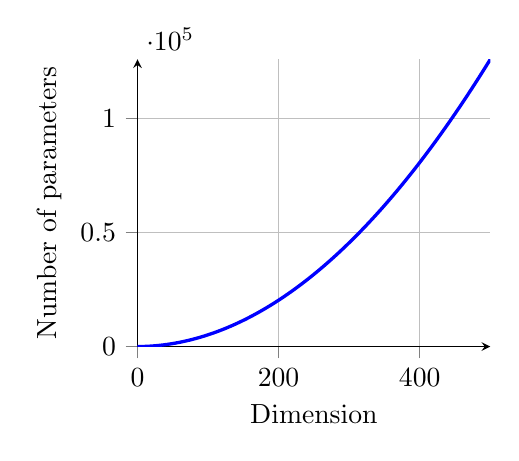
\begin{tikzpicture}
            \begin{axis}[xmin=0,xmax=500,ymin=0,width=0.5*\columnwidth,grid,axis x line=left ,axis y line=left, tick align=outside,xlabel = Dimension,ylabel =Number of parameters]
                \addplot+[very thick,mark=none,smooth,domain=0:500,samples=500] (\x,{\x*(\x+3)/2+1});
            \end{axis}
        \end{tikzpicture}
        \caption{Number of parameters by class in function of dimension.\label{fig:nb-param}}
    \end{figure}

    A lack of samples induces badly-conditioned covariance matrices and so unstable inversion and computation of the determinant. There are two major solutions to this problem. First option is to use a regularization method to stabilize the inversion of the covariance matrices\cite{hoerl1970ridge}. Second option is to use a features extraction/selection method in order to reduce the dimensionality of the samples. In this study, the latter option is explored and a feature selection method named sequential forward features selection is presented in the next Section.

    \subsection{Features selection}
    \label{sec:selection}

    The objective of feature selection is to retrieve the most compact representation of the data with minimum loss of information. In deleting the redundant information, feature selection allows to reduce dimension and thus avoid statistical issue, increase algorithm speed and limit storage requirements. Moreover, it adds several beneficial side effects. It improves data understanding by identify where is the most relevant information and it is then possible to save resources when organizing a new data acquisition.

    It is important to underline that the proposed method is a \emph{selection} method and not an \emph{extraction} method. It means the subset of variables obtained is composed of actual variables of the original set and not variables built as combination of several others as it is the case for example with PCA. This choice is made to assure an easier interpretation by the user of the obtained subset of variables.

    Features selection algorithms may be divided into three types. The first type called filter method is based uniquely on data analysis. Features are ranked according to a statistical analysis of the data. For example, the Principal Component Analysis (PCA) described in \cite{jimenez1998supervised} is a typical filter method and there is numerous other methods \cite{bruzzone1995extension}, \cite{biesiada2007feature}, \cite{demir2008phase}.

    The second sort are known as wrapper methods which can be seen as search method to determine the best subset of variables for a given learning model. As exhaustive searches are out of question in a practical amount of time, numerous search strategies have been designed some optimal under particular hypothesis \cite{narendra1977branch} and other suboptimal but easier to set up \cite{whitney1971direct}, \cite{somol1999adaptive}. The advantage of such methods compare to filter methods is that they are dedicated to a particular model but on the other hand, as they require the training of multiple models to test various set of variables, they tend to be slower.

    The third type corresponds to the embedded method which do not separate the features selection process from the learning algorithm and allow interaction between the two processes. The basic example of such method is the decision tree algorithm in which a feature is selected for the creation of each node. Embedded methods also exist for other models, e.g. SVM \cite{guyon2002gene} \cite{weston2003use}.
²
    The selection method proposed in this work is a wrapper method associated to GMM models. Thus, in order to set a wrapper method, two elements are needed, a function to rank the various features which is defined in Section~\ref{sec:criterion} and a search strategy. Two search algorithms are presented: the sequential forward features selection method (Section \ref{sec:forward-presentation}) and the sequential floating forward feature selection method (\ref{sec:floating-presentation}) the second being a more complex variation of the first.

        \subsubsection{Criterion function}
        \label{sec:criterion}

        \hspace{0pt} \\

        Criterion functions aim to evaluate either a rate of correct classification or the separability/similarity of class distributions. These functions are used to estimate which sets of variables are the best to represent data, to assure the separability of the classes and to perform classification. The choice of a criterion function is the choice of a way to compare sets of variables.

            \paragraph{Measures of correct classification}
            \label{sec:criterion-rate}

            \hspace{0pt} \\

            As described in \cite{congalton2008assessing} (chapter 4), all this measures of good classification are based on an error matrix $M$ called confusion matrix which is defined so that $M_{ij}$ is the number of samples of class $i$ classified as class $j$. The confusion matrix allows the computation of several interesting values relatively to each class:
            \begin{itemize}
                \item the number of True Positive (TP) corresponding to good prediction;
                \item the number of True Negative (TN) corresponding to good classification of the other class;
                \item the number of False Negative (FN) corresponding to the samples of the class labeled as an other class;
                \item the number of False Positive (FP) corresponding to the samples wrongly classified as part of of this class.
            \end{itemize}
            Figure~\ref{fig:confusion} illustrates the definition of this values.

            \begin{figure}[!ht]
                \centering
                \begin{tabular}{c >{\bfseries}r @{\hspace{0.7em}}c @{\hspace{0.4em}}c @{\hspace{0.4em}}c @{\hspace{0.7em}}l}
                  \multirow{10}{*}{\parbox{1.1cm}{\bfseries\raggedleft Actual\\ value}} &
                    & \multicolumn{3}{c}{\bfseries Prediction outcome} \\
                  & & \bfseries $c_1$ & \bfseries $c_2$ & \bfseries $c_3$ \\
                  & $c_1'$ & \MyBox{True}{Positive} & \MyBox{False}{Negative} & \MyBox{False}{Negative} \\[2.4em]
                  & $c_2'$ & \MyBox{False}{Positive} & \MyBox{True}{Negative} & \MyBox{~}{~} \\[2.4em]
                  & $c_3'$ & \MyBox{False}{Positive} & \MyBox{~}{~} & \MyBox{True}{Negative}
                \end{tabular}
                \caption{Confusion matrix with TP, TN, FP and FN relatively to $c_1$}
                \label{fig:confusion}
            \end{figure}

            \emph{The overall accuracy} (OA) is the rate of the number of samples with the correct predicted label over the total number of samples. This metric is easy to interpret but is biased in the case of unbalanced classes.

            \emph{The Cohen's kappa} (K) is a statistic which measures the probability of agreement between predictions and ground-truth.

            \emph{The mean F1 score} (F1mean) is the average of the F1 score for each class and the F1 score is the harmonic mean of the precision (number of True Positive over True Positive plus False Positive) and the recall (number of True Positive over True Positive plus False Negative).

            \begin{align}
                OA &= \frac{\text{TP}}{n}. \\
                K &= \frac{pa - pr}{1 - pr}.  \\
                \text{F1mean} &= \frac{2 \text{TP}}{2 \text{TP} + \text{FN} + \text{FP}}.
            \end{align}
            where TP stands for True Positive, FN for False Negative, FP for False Positive, $pa$ is the probability of agreement defined by $pa = OA$  and $pr$ the probability of random agreement defined by $pr = \sum_{c=1}^{C} \frac{TP_c}{FP_c} \frac{TP_c}{FN_c}$.

            In order to estimate classification rate, a cross-validation process over training set is used\cite{opac-b1127878}. The training set is divided in k folds, then, the training is done with $(k-1)$ folds and the performances are estimated with the remaining fold.

            \hspace{0pt} \\

            \paragraph{Similarity between distributions}

            \hspace{0pt} \\
            The second type of criterion functions is a measure of similarity between two distributions. These measures are called divergence function and are defined so that, if $S$ is a space of all probability distribution with same support, it satisfies
            \begin{align*}
                &\forall (p,q) \in S, \text{Div}(p,q) \geq 0, \\
                &\text{Div}(p,q) = 0 \Leftrightarrow p = q.
            \end{align*}
            More specifically, focus is made on two particular divergences: the Kullback–Leibler divergence and the Jeffries–Matusita distance. The advantage of these divergences is that they have an explicit expression in the case of Gaussian models. The simplification allows to get rid of any integration calculus which is a major problem when dealing with high-dimensional data.


            \emph{The Kullback-Leibler divergence} (KL divergence) measures the amount of information lost when the first distribution is approximated by the second one\cite{kullback1987letter}. The formal definition is
            \begin{equation}
                \text{Div}_{KL}(c_i,c_j) = \int_\mathbf{x} p(\mathbf{x}|c_i) \ln \left(\frac{p(\mathbf{x}|c_i)}{p(\mathbf{x}|c_j)}\right) d\mathbf{x}.
            \end{equation}
            And in the case of Gaussian model, it can be rewritten as follows
            \begin{align}
                &\text{Div}_{KL}(c_i,c_j) = \frac{1}{2} \biggl( \text{Tr} (\boldsymbol{\Sigma}_{c_i}^{-1} \boldsymbol{\Sigma}_{c_j}) \nonumber \\
                & + (\boldsymbol{\mu}_{c_i} - \boldsymbol{\mu}_{c_j})^t \boldsymbol{\Sigma}_{c_i}^{-1} (\boldsymbol{\mu}_{c_i} - \boldsymbol{\mu}_{c_j}) - d + \log \left( \frac{|\boldsymbol{\Sigma}_{c_i}|}{|\boldsymbol{\Sigma}_{c_j}|} \right) \biggr),
            \end{align}
            where Tr is the trace operator and $d$ the dimension of the distribution.

            It can be noticed that the KL divergence is not symmetric, i.e. $\text{Div}_{KL}(c_i,c_j) \ne \text{Div}_{KL}(c_j,c_i)$, and so the symmetrized version is used to compute the criterion function. In the case of Gaussian model, the symmetrization induces the following simplification of the formula
            \begin{align}
                \text{SKL}_{ij} &=\text{Div}_{KL}(c_i,c_j) + \text{Div}_{KL}(c_j,c_i) \nonumber \\
                &= \frac{1}{2} \biggl( \text{Tr} (\boldsymbol{\Sigma}_{c_i}^{-1} \boldsymbol{\Sigma}_{c_j} + \boldsymbol{\Sigma}_{c_j}^{-1} \boldsymbol{\Sigma}_{c_i}) \nonumber \\
                &~~+ (\boldsymbol{\mu}_{c_i} - \boldsymbol{\mu}_{c_j})^t (\boldsymbol{\Sigma}_{c_i}^{-1} + \boldsymbol{\Sigma}_{c_j}^{-1}) (\boldsymbol{\mu}_{c_i} - \boldsymbol{\mu}_{c_j}) - 2d \biggr).
            \end{align}

            Moreover, the divergence is computed between two classes and to obtain a unique value the weighted mean of divergence measures is taken as proposed in \cite{bruzzone1995extension}:
            \begin{equation}
                \text{C}_{SKL} = \sum_{i=1}^{C} \sum_{j=i + 1}^{C} \pi_{c_i} \pi_{c_j} \text{SKL}_{ij}.
            \end{equation}

            \emph{The Bhattacharyya distance} is defined as follows
            \begin{equation}
                \text{B}_{ij} = - \ln \left( \int_\mathbf{x} \sqrt{p(\mathbf{x}|c_i) p(\mathbf{x}|c_j)} d\mathbf{x} \right).
            \end{equation}
            And in the case of Gaussian model:
            \begin{align}
                \text{B}_{ij} = &\frac{1}{8} (\boldsymbol{\mu}_i - \boldsymbol{\mu}_j)^t \left( \frac{\boldsymbol{\Sigma}_i + \boldsymbol{\Sigma}_j}{2} \right)^{-1} (\boldsymbol{\mu}_i - \boldsymbol{\mu}_j) \nonumber \\
                &+ \frac{1}{2} \ln \left( \frac{|\boldsymbol{\Sigma}_i + \boldsymbol{\Sigma}_j|}{\sqrt{|\boldsymbol{\Sigma}_i| |\boldsymbol{\Sigma}_j|}} \right).
            \end{align}

            \emph{The Jeffries–Matusita distance} is a measure based on the Bhattacharyya distance. It saturates if the separability between the two distribution increases \cite{bruzzone2009novel}. The JM distance is defined according to
            \begin{equation}
                \text{JM}_{ij} = \sqrt{ \int_\mathbf{x} \left[\sqrt{p(\mathbf{x}|c_i)} - \sqrt{p(\mathbf{x}|c_j)}\right]^2 d\mathbf{x} }.
            \end{equation}
            And the Jeffries–Matusita distance can be rewritten according to the Bhattacharyya distance
            \begin{equation}
                \text{JM}_{ij} = \sqrt{ 2 \{1 - \text{exp}[-B_{ij}]\} }.
            \end{equation}

            As for the KL divergence, a weighted mean of the distance between two classes is computed to aggregate the measures in a single value:
            \begin{equation}
                \text{C}_{JM} = \sum_{i=1}^{C} \sum_{j=i + 1}^{C} \pi_{c_i} \pi_{c_j} \text{JM}_{ij}.
            \end{equation}

            \vspace{10 mm}

            According to \cite{bruzzone2009novel}, it is interesting to notice that the KL divergence increases quadratically with respect to the distance between the mean vectors of the class distributions whereas the measures of correct classification asymptotically tends to one when distributions are perfectly separable. On the contrary, the JM distance tends to saturate as the measures of correct classification. Table~\ref{tab:crit} summarized the presented criterion functions and their characteristics.

            \begin{table}[!t]
                \centering
                \caption{Summary of the various criterion functions.\label{tab:crit}}
                \begin{tabular}[b]{l|c|c||c|c}
                  \hline
                  Criterion & Divergence & Classification rate & Gaussian hypothesis & Speed \\
                  \hline
                  Overall accuracy            &  & \checkmark & 0 & - \\
                  Cohen's kappa               &  & \checkmark & 0 & - \\
                  F1 mean                     &  & \checkmark & 0 & - \\
                  Kullback-Leibler divergence & \checkmark &  & ++ & + \\
                  Jeffries-Matusita distance  & \checkmark &  & ++ & + \\
                  \hline
                \end{tabular}
            \end{table}

        \subsubsection{Selection method}

            \paragraph{Sequential forward features selection}
            \label{sec:forward-presentation}

            The Sequential Forward Selection (SFS) starts with an empty set of selected features. Then, it computes at each step for all the remaining features the value of the criterion function $J$ chosen among the ones presented in Table~\ref{tab:crit} when the feature is added to the pool of selected features. The feature that maximizes the criterion function is definitively added to the pool of selected features and it moves to the next iteration. The algorithm stops when a given number of variables \emph{maxVarNb} has been selected. The Algorithm~\ref{alg:sfs} presents the process in details.

            The advantage of this search algorithm is its reasonable processing time. The trade-off is that the result is a suboptimal solution in the sense that an untested subset of variable could lead to better classification result.

            \begin{algorithm}
            \caption{Sequential forward features selection\label{alg:sfs}}
            {\footnotesize
            \begin{algorithmic}[1]
            \REQUIRE $\Omega,J,\text{maxVarNb}$
            \STATE $\Omega=\emptyset$
            \STATE $F=\text{\{all variables\}}$
            \WHILE{$\text{card}(\Omega) \leq maxVarNb$}
            \FORALL{$f_i \in F$}
            \STATE $R_i = J(\{\Omega + f_i\})$
            \ENDFOR
            \STATE $j=\text{arg} \max_{i} R_i$
            \STATE $\Omega = \{\Omega + f_j\}$
            \STATE $F = F \setminus f_j$
            \ENDWHILE
            \RETURN $\Omega$
            \end{algorithmic}
            }
            \end{algorithm}

            \paragraph{Sequential floating forward feature selection}
            \label{sec:floating-presentation}

            The Sequential Floating Forward Selection (SFFS) is actually based on two algorithms: the SFS described above and the Sequential Backward Selection (SBS). The SBS is the backward equivalent of SFS. The difference is that it starts with every features in the pool of selected features and tries at each step to remove the less significant one in term of the given criterion function.

            The SFFS works as the SFS but between each step of the SFS algorithm a backward selection is operated. At the end of the SBS step, the value of the criterion function is compared to the best value ever obtained with a set of features of the same size and if the new value is better the feature put into question is effectively taken away and the next step is again a SBS but if the new value is not better the SBS step is forgotten and it moves to the next SFS step. The algorithm stops when a given number of features \emph{maxVarNb} has been selected. The Algorithm~\ref{alg:sffs} sums up the method.

            This SFFS algorithm eventually tests more solutions than the SFS algorithm. The results are expected to be better but the trade-off is an increased computational time which is dependent on the complexity of the dataset.

            \begin{algorithm}
            \caption{Sequential floating forward features selection\label{alg:sffs}}
            {\footnotesize
            \begin{algorithmic}[1]
            \REQUIRE $\Omega,J,\text{maxVarNb}$
            \STATE $\Omega=\emptyset$
            \STATE $F=\text{\{all variables\}}$
            \STATE $k=0$
            \WHILE{$\text{card}(\Omega) \leq maxVarNb$}
            \FORALL{$f_i \in F$}
            \STATE $R_i = J(\{\Omega{(k)} + f_i\})$
            \ENDFOR
            \STATE $j=\text{arg} \max_{i} R_i$
            \IF{$R_j \geq J(\Omega^{(k+1)})$}
            \STATE $k=k+1$
            \ELSE
            \STATE $\Omega^{(k+1)} = \{\Omega{(k)} + f_i\}$
            \STATE $k=k+1$
            \STATE $\text{flag}=1$
            \WHILE{$k > 2 \text{ and } \text{flag}=1$}
            \FORALL{$f_i \in \Omega^{(k)}$}
            \STATE $R_i = J(\{\Omega{(k)}\setminus f_i\})$
            \ENDFOR
            \STATE $j=\text{arg} \max_{i} R_i$
            \IF{$R_j < J(\Omega^{(k-1)})$}
            \STATE $\Omega^{(k-1)} = \{\Omega{(k)} \setminus f_i\}$
            \STATE $k=k-1$
            \ELSE
            \STATE $\text{flag}=0$
            \ENDIF
            \ENDWHILE
            \ENDIF
            \ENDWHILE
            \RETURN $\Omega$
            \end{algorithmic}
            }
            \end{algorithm}


\section{Efficient implementation}
\label{sec:implementation}

    \subsection{Statistical update rules}
    A major contribution of this work is the optimization in term of computational efficiency. More precisely, three steps of the proposed method has been upgraded in order to reduce computational time. First of all, the GMM model is learned only once using samples. When a covariance matrix or a mean vector of a reduced set of variables is required, it is obtained from the global model learned at the beginning by marginalization.

    Secondly, when a cross-validation is performed, submodels, i.e. GMM model trained with $(n-1)$ folds, are not learned using the $(n-1)$ folds but, instead, are derived from the global model and from the covariance matrices and mean vectors of the fold used for validation for the given submodel. The process is described in details in Section~\ref{sec:update-cv}.

    Finally and most importantly, when variables are tested one by one during a selection step, costly operations are made when computing criterion functions for each variable especially the computation of the inverse of covariance matrices and its determinant. Several update rules are set up which allow to compute this inverse and determinant only once to test all variables. These update rules are presented in Section~\ref{sec:update-crit}.

        \subsubsection{Update for cross validation}
        \label{sec:update-cv}

        Based on \cite{fauvel2015fast}, a method to accelerate the $n_{cv}$-fold cross-validation process in the case of criterion functions based on correct classification measures was implemented. The idea is to estimate the GMM model with the whole training set and then, instead of training a model on $(n_{cv}-1)$ folds, the complete model and the mean vector and the covariance matrix of the $k^{th}$ fold is used to derive the corresponding submodel.

        The following formulae can be obtained
        \begin{prop}
            \label{eq:update-cv1}
            (Cross-validation mean update)
            \begin{equation*}
                \boldsymbol{\mu}_c^{n_c-\nu_c} = \frac{n_c \boldsymbol{\mu}_c^{n_c} - \nu_c \boldsymbol{\mu}_c^{\nu_c}}{n_c - \nu_c} \nonumber
            \end{equation*}
        \end{prop}
        \begin{prop}
            \label{eq:update-cv2}
            (Cross-validation covariance matrix update)
            \begin{align*}
                \boldsymbol{\Sigma}_c^{n_c-\nu_c} = &\frac{1}{n_c-\nu_c-1} \biggl( (n_c-1) \boldsymbol{\Sigma}_c^{n_c} - (\nu_c-1) \boldsymbol{\Sigma}_c^{\nu_c} \nonumber \\
                &- \frac{n_c \nu_c}{(n_c-\nu_c)} (\boldsymbol{\mu}_c^{\nu_c}-\boldsymbol{\mu}_c^{n_c})(\boldsymbol{\mu}_c^{\nu_c}-\boldsymbol{\mu}_c^{n_c})^t \biggr) \nonumber
            \end{align*}
        \end{prop}
        where $\nu_c$ is the number of samples of class $c$ removed from the initial set, $\boldsymbol{\mu}_c^{n_c}$ the mean vector estimated with this $\nu_c$ samples and $\boldsymbol{\Sigma}_c^{\nu_c}$ the covariance matrix estimated with this $\nu_c$ samples.

        \subsubsection{Criterion function computation}
        \label{sec:update-crit}

        As explained earlier, at each iteration the SFS and SFFS algorithms compute the value of a criterion function for every possible set of features composed of the selected ones augmented by one of the remaining features. One of the main achievements of this work is to reduce the computational time needed to compute the criterion function of augmented sets.

        In the remaining of the paper, $\boldsymbol{\Sigma}^{(k-1)}$ is the covariance matrix of the $(k-1)^{th}$ iteration, i.e., the covariance matrix of the selected features and $\boldsymbol{\Sigma}^{(k)}$ is a covariance matrix at the $k^{th}$ iteration, i.e., the covariance matrix of an augmented set. Then, the inverse of the covariance matrix $(\boldsymbol{\Sigma}^{(k)})^{-1}$, the quadratical term $(\mathbf{x}^{(k)})^t (\boldsymbol{\Sigma}^{(k)})^{-1} \mathbf{x}^{(k)}$ and the determinant $\log |\boldsymbol{\Sigma}^{(k)}|$ can be expressed in function of terms of the $(k-1)^{th}$ iteration. These calculi use the fact that the covariance matrix is a positive definite symmetric matrix to simplify formulae using block matrices \cite{webb2003statistical} (chapter 9.2). These update rules are summed up hereafter

        In order to easily understand which terms are available and which ones needs to be computed, the terms already computed are set in green in the update rules.

        As $\boldsymbol{\Sigma}^{(k)}$ is a positive definite symmetric matrix, the following notation can be used
        \begin{equation*}
            \boldsymbol{\Sigma}^{(k)} =
            \bigg[\begin{array}{cc}
            \boldsymbol{\Sigma}^{(k-1)} & \mathbf{u}      \\
            \mathbf{u}^t          & \sigma_{kk} \\
            \end{array}\bigg],
        \end{equation*}
        where $\mathbf{u}$ is the $k^{th}$ column of the matrix without the diagonal element i.e. $\mathbf{u}_{i} = \boldsymbol{\Sigma}^{(k)}_{i,k}$ with $i \in [1,k-1]$.

        Using the formula of the inverse of a block matrix, the following formula expressing $(\boldsymbol{\Sigma}^{(k)})^{-1}$ in function of $(\boldsymbol{\Sigma}^{(k-1)})^{-1}$ is obtained
        \begin{prop}
        \label{eq:update-inv}
            (Forward update rule for inverse of covariance matrix)
            \begin{equation*}
                \fbox{$
                (\boldsymbol{\Sigma}^{(k)})^{-1} =
                \bigg[\begin{array}{cc}
                A & v \\
                v^t  & \frac{1}{\alpha} \\
                \end{array}\bigg]
                $}
            \end{equation*}
        \end{prop}
        where $A = \textcolor[rgb]{0,0.5,0}{(\boldsymbol{\Sigma}^{(k-1)})^{-1}} + \frac{1}{\alpha} \textcolor[rgb]{0,0.5,0}{(\boldsymbol{\Sigma}^{(k-1)})^{-1}} \mathbf{u} \mathbf{u}^t \textcolor[rgb]{0,0.5,0}{(\boldsymbol{\Sigma}^{(k-1)})^{-1}}$, $v = - \frac{1}{\alpha} \textcolor[rgb]{0,0.5,0}{(\boldsymbol{\Sigma}^{(k-1)})^{-1}} \mathbf{u}$ and $ \alpha = \sigma_{kk} - \mathbf{u}^t \textcolor[rgb]{0,0.5,0}{(\boldsymbol{\Sigma}^{(k-1)})^{-1}} \mathbf{u} $.

        It means that, to select a variable among one hundred, instead of computing one hundred times $(\boldsymbol{\Sigma}^{(k)})^{-1}$, $(\boldsymbol{\Sigma}^{(k-1)})^{-1}$ is computed once and then with a few matrix multiplications and sums, the hundred inverses are obtained and a lot of processing time is saved.

        In the case of a backward step in SFFS algorithm, the formula is inverted in order to compute $(\boldsymbol{\Sigma}^{(k-1)})^{-1}$ knowing $(\boldsymbol{\Sigma}^{(k)})^{-1}$. The update rule becomes
        \begin{prop}
            (Backward update rule for inverse of covariance matrix)
            \begin{equation*}
                \fbox{$(\boldsymbol{\Sigma}^{(k-1)})^{-1} = \textcolor[rgb]{0,0.5,0}{\mathbf{A}} - \alpha \mathbf{v} \mathbf{v}^t$}
            \end{equation*}
        \end{prop}

        \begin{proof}
            \begin{align*}
                \mathbf{A} - \alpha \mathbf{v} \mathbf{v}^t
                &= (\boldsymbol{\Sigma}^{(k-1)})^{-1} + \frac{1}{\alpha} (\boldsymbol{\Sigma}^{(k-1)})^{-1} \mathbf{u} \mathbf{u}^t (\boldsymbol{\Sigma}^{(k-1)})^{-1} \\
                &~~~- \alpha (- \frac{1}{\alpha} (\boldsymbol{\Sigma}^{(k-1)})^{-1} \mathbf{u}) (- \frac{1}{\alpha} \mathbf{u}^t (\boldsymbol{\Sigma}^{(k-1)})^{-1})) \\
                &= (\boldsymbol{\Sigma}^{(k-1)})^{-1}
            \end{align*}
        \end{proof}

        A formula can also be deduced for the quadratical term of the decision function. Noting $(\mathbf{x}^{(k)})^t = \left[\begin{array}{cc} (\mathbf{x}^{(k-1)})^t   & x^k \end{array}\right]$, the following proposition is obtained
        \begin{prop}
        \label{eq:update-quad}
            (Update rule for quadratical term)
            \begin{empheq}[box=\fbox]{align*}
                (\mathbf{x}^{(k)})^t (\boldsymbol{\Sigma}^{(k)})^{-1} \mathbf{x}^{(k)} = &\textcolor[rgb]{0,0.5,0}{(\mathbf{x}^{(k-1)})^t (\boldsymbol{\Sigma}^{(k-1)})^{-1} \mathbf{x}^{(k-1)}} \\
                &+ \alpha ( \left[\begin{array}{cc} \mathbf{v}^t & \frac{1}{\alpha} \end{array}\right] \mathbf{x}^{(k)} )^2
            \end{empheq}
        \end{prop}

        \begin{proof}
            \begin{align*}
                (&\mathbf{x}^{(k)})^t (\boldsymbol{\Sigma}^{(k)})^{-1} \mathbf{x}^{(k)}
                = \left[\begin{array}{cc} (\mathbf{x}^{(k-1)})^t   & x_k \end{array}\right]
                \left[\begin{array}{cc}
                \mathbf{A}   & \mathbf{v} \\
                \mathbf{v}^t & \frac{1}{\alpha}
                \end{array}\right]
                \left[\begin{array}{c} \mathbf{v} \\ x_k \end{array}\right] \\
                &= \left[\begin{array}{cc} (\mathbf{x}^{(k-1)})^t \mathbf{A} + x_k \mathbf{v}^t & (\mathbf{x}^{(k-1)})^t \mathbf{v} + \frac{x_k}{\alpha} \end{array}\right]
                \left[\begin{array}{c} \mathbf{v} \\ x_k \end{array}\right] \\
                &= (\mathbf{x}^{(k-1)})^t \mathbf{A} \mathbf{x}^{(k-1)} + x_k \mathbf{v}^t \mathbf{x}^{(k-1)} + (\mathbf{x}^{(k-1)})^t \mathbf{v} x_k + \frac{(x_k)^2}{\alpha} \\
                &= (\mathbf{x}^{(k-1)})^t ((\boldsymbol{\Sigma}^{(k-1)})^{-1} + \frac{1}{\alpha} (\boldsymbol{\Sigma}^{(k-1)})^{-1} \mathbf{u} \mathbf{u}^t (\boldsymbol{\Sigma}^{(k-1)})^{-1}) \mathbf{x}^{(k-1)}\\
                &~~~+ 2 x_k \mathbf{v}^t \mathbf{x}^{(k-1)} + \frac{(x_k)^2}{\alpha} \\
                &= (\mathbf{x}^{(k-1)})^t ((\boldsymbol{\Sigma}^{(k-1)})^{-1} + \alpha \mathbf{v} \mathbf{v}^t) \mathbf{x}^{(k-1)}\\
                &~~~+ 2 x_k \mathbf{v}^t \mathbf{x}^{(k-1)} + \frac{(x_k)^2}{\alpha} \\
                &= (\mathbf{x}^{(k-1)})^t (\boldsymbol{\Sigma}^{(k-1)})^{-1} \mathbf{x}^{(k-1)} + \alpha ( (\mathbf{x}^{(k-1)})^t \mathbf{v} \mathbf{v}^t \mathbf{x}^{(k-1)} \\
                &~~~+ 2 \frac{x_k}{\alpha} \mathbf{v}^t \mathbf{x}^{(k-1)} + \frac{(x_k)^2}{\alpha^2}) \\
                &= (\mathbf{x}^{(k-1)})^t (\boldsymbol{\Sigma}^{(k-1)})^{-1} \mathbf{x}^{(k-1)} + \alpha ( (\mathbf{x}^{(k-1)})^t \mathbf{v} + \frac{x_k}{\alpha} )^2 \\
                &= (\mathbf{x}^{(k-1)})^t (\boldsymbol{\Sigma}^{(k-1)})^{-1} \mathbf{x}^{(k-1)} + \alpha ( \left[\begin{array}{cc} \mathbf{v}^t & \frac{1}{\alpha} \end{array}\right] \mathbf{x}^{(k)} )^2
            \end{align*}
        \end{proof}

        Finally, using the formula of the determinant of a block matrix and after taking the log, a last formula is produced
        \begin{prop}
        \label{eq:update-log}
            (Update rule for logdet)
            \begin{equation*}
                \fbox{$\log \left(|\boldsymbol{\Sigma}^{(k)}|\right) = \textcolor[rgb]{0,0.5,0}{\log \left(|\boldsymbol{\Sigma}^{(k-1)}|\right)} + \log \alpha$}
            \end{equation*}
        \end{prop}

        Now using all update rules, criterion functions can be rewritten as follows
        \begin{align}
        \label{eq:q-update}
            Q(\mathbf{x}) = &- \textcolor[rgb]{0,0.5,0}{(\mathbf{x}^{(k-1)} - \boldsymbol{\mu}^{(k-1)})^t (\boldsymbol{\Sigma}^{(k-1)})^{-1} (\mathbf{x}^{(k-1)} - \boldsymbol{\mu}^{(k-1)})} \nonumber \\
            &- \alpha \left( \left[\begin{array}{cc} \mathbf{v}^t & \frac{1}{\alpha} \end{array}\right] (\mathbf{x}^{(k)} - \boldsymbol{\mu}^{(k)}) \right)^2 \nonumber \\
            &- \textcolor[rgb]{0,0.5,0}{\log \left(|\boldsymbol{\Sigma}^{(k-1)}|\right)} - \log \alpha  + \textcolor[rgb]{0,0.5,0}{2 \log (\pi_c)} + \textcolor[rgb]{0,0.5,0}{k \log(2 \pi)};
        \end{align}

        {\footnotesize
        \begin{align}
        \label{eq:skl-update}
            &\text{SKL}_{ij} = \frac{1}{2} \biggl( \text{Tr} \left((\boldsymbol{\Sigma}_{c_i}^{(k)})^{-1} \boldsymbol{\Sigma}_{c_j}^{(k)} + (\boldsymbol{\Sigma}_{c_j}^{(k)})^{-1} \boldsymbol{\Sigma}_{c_i}^{(k)}\right) \nonumber \\
            &+ \textcolor[rgb]{0,0.5,0}{(\boldsymbol{\mu}_{c_i}^{(k-1)} - \boldsymbol{\mu}_{c_j}^{(k-1)})^t ((\boldsymbol{\Sigma}_{c_i}^{(k-1)})^{-1} + (\boldsymbol{\Sigma}_{c_j}^{(k-1)})^{-1}) (\boldsymbol{\mu}_{c_i}^{(k-1)} - \boldsymbol{\mu}_{c_j}^{(k-1)})} \nonumber \\
            &+ \alpha ( \left[\begin{array}{cc} \mathbf{v_i}^t & \frac{1}{\alpha_i} \end{array}\right] (\boldsymbol{\mu}_{c_i}^{(k)} - \boldsymbol{\mu}_{c_j}^{(k)}) )^2 \nonumber \\
            &+ \alpha ( \left[\begin{array}{cc} \mathbf{v_j}^t & \frac{1}{\alpha_j} \end{array}\right] (\boldsymbol{\mu}_{c_i}^{(k)} - \boldsymbol{\mu}_{c_j}^{(k)}) )^2
            - \textcolor[rgb]{0,0.5,0}{2k} \biggr),
        \end{align}
        }
        with $(\boldsymbol{\Sigma}_{c_i}^{(k)})^{-1}$ computed with Proposition~\ref{eq:update-inv};

        \begin{align}
        \label{eq:jm-update}
            \text{B}_{ij} = &\textcolor[rgb]{0,0.5,0}{\frac{1}{4} (\boldsymbol{\mu}_i^{(k-1)} - \boldsymbol{\mu}_j^{(k-1)})^t ( \boldsymbol{\tilde{\Sigma}}^{(k-1)} )^{-1} (\boldsymbol{\mu}_i^{(k-1)} - \boldsymbol{\mu}_j^{(k-1)})} \nonumber \\
            &+ \frac{1}{4} \tilde{\alpha} ( \left[\begin{array}{cc} \mathbf{\tilde{v}}^t & \frac{1}{\tilde{\alpha}} \end{array}\right] (\boldsymbol{\mu}_{i}^{(k)} - \boldsymbol{\mu}_{j}^{(k)}) )^2 \nonumber \\
            &+ \textcolor[rgb]{0,0.5,0}{\frac{1}{2} \ln \left( \frac{|\boldsymbol{\tilde{\Sigma}}^{(k-1)}|}{\sqrt{|\boldsymbol{\Sigma}_i^{(k-1)}| |\boldsymbol{\Sigma}_j^{(k-1)}|}} \right)} + \frac{1}{2} \ln \left( \frac{\tilde{\alpha}}{\sqrt{\alpha_i \alpha_j}} \right),
        \end{align}
        where $\boldsymbol{\tilde{\Sigma}} = \boldsymbol{\Sigma}_i + \boldsymbol{\Sigma}_j$.

        The Algorithm~\ref{alg:sffs-update} illustrates the optimization of the Algorithm~\ref{alg:sffs} developed using these formulae.

    \subsection{Numerical issues}

    During an iteration of the selection algorithm, it still needs to invert the covariance matrix of the previous iteration. In order to so, a decomposition in eigenvalues and eigenvectors is performed using algorithm specific for symmetric matrices. More precisely, In other words, $\boldsymbol{\Sigma}$ is decomposed s.t. $\boldsymbol{\Sigma} = \mathbf{Q} \boldsymbol{\Lambda} \mathbf{Q}^t$ with $\boldsymbol{\Lambda}$ the diagonal matrix of eigenvalues and $\mathbf{Q}$ the matrix of eigenvectors.

    This decomposition has several advantages. First, it is very simple to compute the determinant once the eigenvalues are available because the determinant is equal to the product of these values. Secondly, it is possible to check the eigenvalues and so to assure a better computational stability. Due to the curse of dimensionality, the covariance matrix is sometimes badly conditioned and the result is that some eigenvalues are really small (below computational precision). The decomposition helps to check their actual values and if they are below EPS\_FLT which is the machine maximum precision for a float, these eigenvalues are set to EPS\_FLT. For the same reason, the constant $\alpha$ used in update rules is also thresholded to EPS\_FLT. Algorithm~\ref{alg:sffs-update} details when computational stability is checked.

    \begin{algorithm}
    \caption{Sequential floating forward features selection with updates\label{alg:sffs-update}}
    {\footnotesize
    \begin{algorithmic}[1]
    \REQUIRE $\Omega,J,\text{maxVarNb}$
    \STATE $\Omega=\emptyset$
    \STATE $F=\text{\{all variables\}}$
    \STATE $k=0$
    \WHILE{$\text{card}(\Omega) \leq maxVarNb$}
    \STATE Diagonalize $\boldsymbol{\Sigma}^{(k-1)} = \mathbf{Q} \boldsymbol{\Lambda} \mathbf{Q}^t$
    \STATE {\bfseries for all} $\lambda_i$ {\bfseries do} $\lambda_i = \min (\text{EPS\_FLT},\lambda_i)$
    \STATE Precompute {\scriptsize $(\boldsymbol{\Sigma}^{(k-1)})^{-1}$, $(\mathbf{x}^{(k-1)} - \boldsymbol{\mu}^{(k-1)})^t (\boldsymbol{\Sigma}^{(k-1)})^{-1} (\mathbf{x}^{(k-1)}- \boldsymbol{\mu}^{(k-1)})$ and $\log \left(|\boldsymbol{\Sigma}^{(k-1)}|\right)$} using Propositions \ref{eq:update-inv}, \ref{eq:update-quad} and \ref{eq:update-log}
    \FORALL{$f_i \in F$}
    \STATE Compute update constant $\alpha$
    \STATE $\alpha = \min (\text{EPS\_FLT},\alpha)$
    \STATE $R_i = J(\{\Omega{(k)} + f_i\})$ using Equations \ref{eq:q-update}, \ref{eq:skl-update} or \ref{eq:jm-update}
    \ENDFOR
    \STATE $j=\text{arg} \max_{i} R_i$
    \IF{$R_j \geq J(\Omega^{(k+1)})$}
    \STATE $k=k+1$
    \ELSE
    \STATE $\Omega^{(k+1)} = \{\Omega{(k)} + f_i\}$
    \STATE $k=k+1$
    \STATE $\text{flag}=1$
    \WHILE{$k > 2 \text{ and } \text{flag}=1$}
    \STATE Diagonalize $\boldsymbol{\Sigma}^{(k-1)} = = \mathbf{Q} \boldsymbol{\Lambda} \mathbf{Q}^t$
    \STATE {\bfseries for all} $\lambda_i$ {\bfseries do} $\lambda_i = \min (\text{EPS\_FLT},\lambda_i)$
    \STATE Compute {\scriptsize $(\boldsymbol{\Sigma}^{(k-1)})^{-1}$, $(\mathbf{x}^{(k-1)} - \boldsymbol{\mu}^{(k-1)})^t (\boldsymbol{\Sigma}^{(k-1)})^{-1} (\mathbf{x}^{(k-1)}- \boldsymbol{\mu}^{(k-1)})$ and $\log \left(|\boldsymbol{\Sigma}^{(k-1)}|\right)$} using Propositions \ref{eq:update-inv}, \ref{eq:update-quad} and \ref{eq:update-log}
    \FORALL{$f_i \in \Omega^{(k)}$}
    \STATE Compute update constant $\alpha$
    \STATE $\alpha = \min (\text{EPS\_FLT},\alpha)$
    \STATE $R_i = J(\{\Omega{(k)}\setminus f_i\})$ using Equations \ref{eq:q-update}, \ref{eq:skl-update} or \ref{eq:jm-update}
    \ENDFOR
    \STATE $j=\text{arg} \max_{i} R_i$
    \IF{$R_j < J(\Omega^{(k-1)})$}
    \STATE $\Omega^{(k-1)} = \{\Omega{(k)} \setminus f_i\}$
    \STATE $k=k-1$
    \ELSE
    \STATE $\text{flag}=0$
    \ENDIF
    \ENDWHILE
    \ENDIF
    \ENDWHILE
    \RETURN $\Omega$
    \end{algorithmic}
    }
    \end{algorithm}

    \subsection{OTB external module}
    \label{sec:otb-module}

    The Orfeo Toolbox is an open-source library for remote sensing image processing. This library allows developers to code external modules and make them available to the community. It is to note that the toolbox already implements several classifiers inherited mostly from OpenCV. Nevertheless, the GMM classifier currently in place is not robust to high dimensionality and that is why a new GMM model has been developed.

    The developed module is available on Github \footnote{\url{https://github.com/Laadr/otbExternalFastFeaturesSelection}} and is a fork of the template for remote module furnished by OTB developers.

    The GMM classifier class called \emph{GMMMachineLearningModel} inherits from the OTB class \emph{MachineLearningModel} which is a basic class used for all classifier in the OTB. The \emph{MachineLearningModel} class enables the management of a list of samples used for training and also declares the virtual methods inherited: \emph{Train()}, \emph{Predict()}, \emph{Save()}, \emph{Load()}.

    The \emph{GMMMachineLearningModel} class implements all these virtual methods. The \emph{Train()} aims to train the classifier using a list of samples set as a class member. Then, it is possible to use the method \emph{Predict()} to classify a sample and optional get the confidence in the prediction. The methods \emph{Save()} and \emph{Load()} obviously are used to save and load a trained model.

    In addition to these inherited methods, two noticeable methods are implemented. The \emph{Decomposition()} method perform a decomposition of a symmetric matrix in eigenvalues and eigenvectors using a function of the VNL library. It is to notice that this method check the value of the extracted eigenvalues and minor them to EPSILON\_FLT (or EPSILON\_DBL) which corresponds to computational precision.  The idea is to limit computational instability when parameters are badly-estimated due to an insufficient amount of training samples. The second interesting method is \emph{TrainTau()} which concerns an optional ridge regularization. Given a set of possible regularization constant $\tau$, this method selects the most efficient value in estimating classification rate with cross-validation.

    To implement the selection algorithm, a new class \emph{GMMSelectionMachineLearningModel} inheriting from \emph{GMMMachineLearningModel} is defined. This class keeps the same six methods inherited from \emph{MachineLearningModel} but reimplements \emph{Predict()} to predict with a reduced set of features and  \emph{Save()}/\emph{Load()} to use a second file to handle the results of the selection.

    The other methods available in class \emph{GMMSelectionMachineLearningModel} are used to perform the selection algorithms presented in Section \ref{sec:gmm-hd}. The method \emph{Selection()} aims to set the various parameter of the selection and then calls either the \emph{ForwardSelection()} method to use forward feature selection or the \emph{FloatingForwardSelection()} method to use SFFS. Then, 3 different methods are used to evaluate criterion functions during selection. Given a pool of variables available for selection, these functions evaluate the criterion functions for all the possible augmented set. The \emph{ComputeJM()} method is used for Jeffries-Matusita distance, \emph{ComputeDivKL()} for Kullback–Leibler divergence and \emph{ComputeClassifRate()} for the three correct classification criteria. It is to notice that the correct classification criteria are evaluated using cross-validation.

    In order to provide an easy way to use the developed algorithm, OTB applications has been developed. These applications allow the user to use and parametrize the algorithm from command line. Three applications are built.

    The application \emph{otbcli\_TrainGMMApp} creates and trains a model from class \emph{GMMMachineLearningModel} and the application \emph{otbcli\_TrainGMMSelectionApp} does the same for a model of class \emph{GMMSelectionMachineLearningModel}. These two applications use a raster image and shapefile with groundtruth as input and create a model file.

    The last application \emph{otbcli\_PredictGMMApp} takes a raster image as input and a model file and perform classification of the image. It generates a classification map in an image file and optionally a confidence map. An other application is available in the OTB to compute classification rate from the image and a groundtruth file.

\section{Experimental results}
\label{sec:test}

    \subsection{Method}
    \label{sec:method}

    The aim of the experiments is to compare the proposed method to some standard classifiers. In order to do it, OTB commandline application are used. The following classifier are tested:
    \begin{itemize}
        \item a k-nearest-neighbors classifier (KNN) with OTB default parameters (32 number of neighbors);
        \item a Random Forest classifier with parameters optimized by gridsearch (200 trees, 40 max depth, 50 size of subset of variables);
        \item a GMM classifier with ridge regularization (GMM ridge) with regularization constant optimized by gridsearch.
    \end{itemize}
    The GMM classifier is part of the external module described in Section~\ref{sec:otb-module}.

    All these classifiers are compared with 3 configurations of the proposed GMM classifier:
    \begin{itemize}
        \item one with forward selection and JM distance as criterion (GMM SFS JM);
        \item one with forward selection and Cohen's kappa as criterion (GMM SFS kappa);
        \item one with floating forward selection and JM distance as criterion (GMM SFFS JM).
    \end{itemize}

    The results obtained with two different datasets are presented. The first dataset is an airborne hyperspectral dataset and second is a remote sensing dataset made of heterogeneous spatial features. Training set has been created with an equal number of samples for each class and additionally a spatial stratification has been performed. Several size of training set has been tested. For Aisa dataset, experiments have been conducted using 250, 500 and 1000 samples by class and for the Potsdam dataset, 1000 and 50000 samples by class.

    For SFS and SFFS selection, the number of variables to select is set to 30 for the Aisa datset and 60 for the Potsdam dataset and then the number of variables which maximizes the criterion function is used to perform classification.

    The classification rate is presented using Cohen's kappa but it has to be noticed the results were similar when looking at the mean F1-score. Processing time has been evaluated on a desktop computer with 4Gb of RAM and Intel(R) Core(TM) i5-3570 CPU \@ 3.40GHz x 4 processor. All results has been estimated with multiple repetitions (20 trials with Aisa dataset, 5 trials with Potsdam dataset).

    \subsection{Aisa dataset}
    \label{sec:aisa}
    The Aisa dataset has been acquired by the AISA Eagle sensor during a flight campaign over Heves, Hungary. It contains 252 bands ranging from 395 to 975 nm. 16 classes have been defined for a total of 361,971 referenced pixels. Figure~\ref{fig:aisa} shows a colored composition of the multispectral image and the shapefile representing groundtruth and Table \ref{tab:aisa} presents the repartition of the various classes.

    \begin{figure}[!t]
        \centering
        \begin{tabular}{c}
            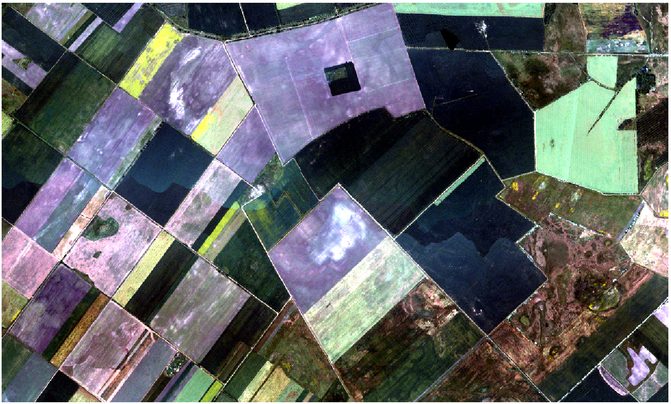
\includegraphics[width=0.7\columnwidth]{Fig/aisa.png} \\
            {\bfseries{(a)}} \\
            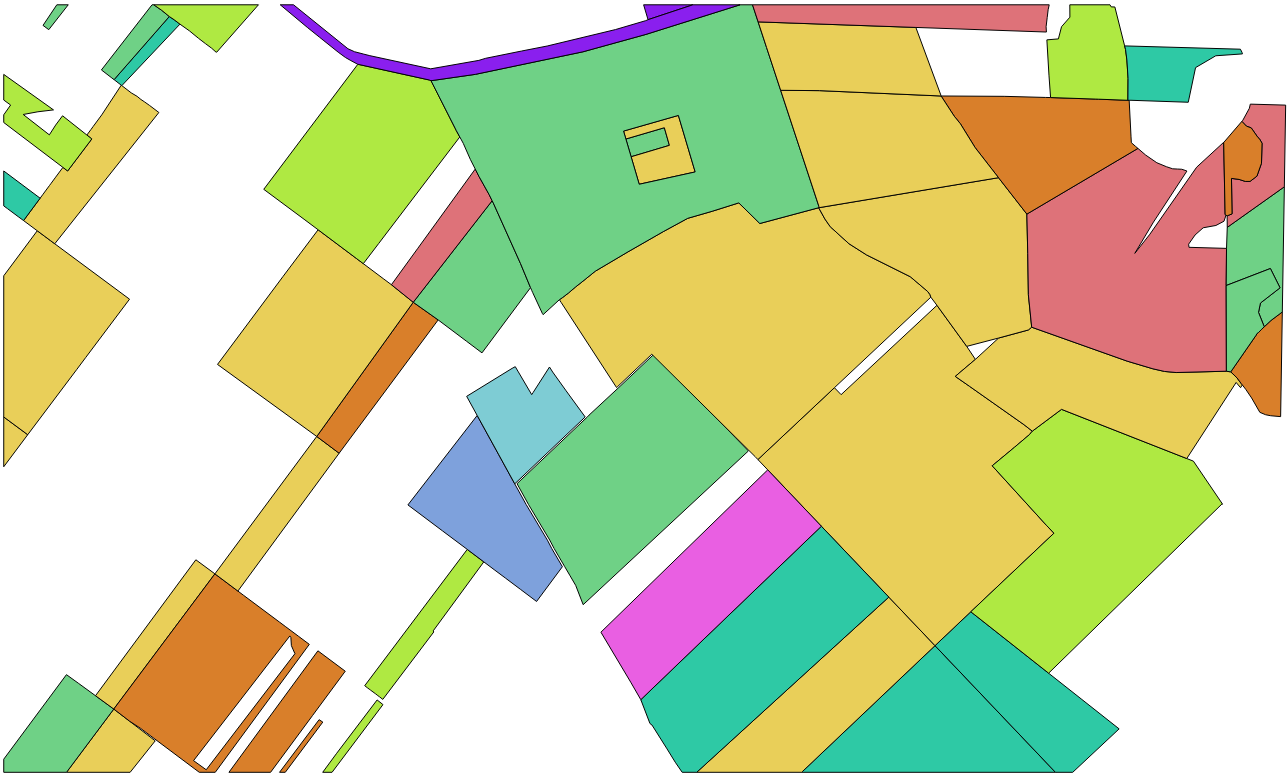
\includegraphics[width=0.7\columnwidth]{Fig/aisa_gt.png} \\
            {\bfseries{(b)}} \\
        \end{tabular}
        \caption{Aisa dataset: {\bfseries{(a)}} colored composition of the image, {\bfseries{(b)}} groundtruth.\label{fig:aisa}}
    \end{figure}

    \begin{table}[!t]
        \centering
        \caption{Repartition of classes in Aisa dataset.\label{tab:aisa}}
        \begin{tabular}[b]{lc}\hline
          Class & Number of samples \\ \hline
          Winter wheat & 136,524 \\
          Sunflower & 61,517 \\
          Green fallow last year treatment & 30,197 \\
          Alfalfa & 17,626 \\
          Maize & 18,278 \\
          Millet & 7,199 \\
          Broadleaved forest & 10,746 \\
          Meadow & 23,283 \\
          Winter barley & 2,799 \\
          Reed & 4,222 \\
          Water course & 4,773 \\
          Rape & 26,566 \\
          Green fallow with shrub & 9,272 \\
          Green fallow last year treated & 3,426 \\
          Pasture & 2,107 \\
          Oat & 3,436 \\ \hline
        \end{tabular}
    \end{table}

    When creating training and validation sets, special care is taken to assure that training samples are picked in distinct areas than test samples. In order to do it, the polygons of the reference are split in smaller polygons and then 50\% of the polygons are taken randomly for training and the remaining 50\% for validation. Moreover 20 trials are run each time with a different training set (different polygons). An example of training and validation set is shown in Figure~\ref{fig:set-aisa}. Additionally, it is important to understand that only a subpart of this training set is actually used to train the model, a given number of samples for each class. Table~\ref{tab:aisa-otbsimu} presents the results of the experiment with mean and standard deviation over the 20 trials and Table~\ref{tab:aisa-otbsimu-time} the corresponding processing time.

    \begin{figure}[!t]
        \centering
        \begin{tabular}{c}
            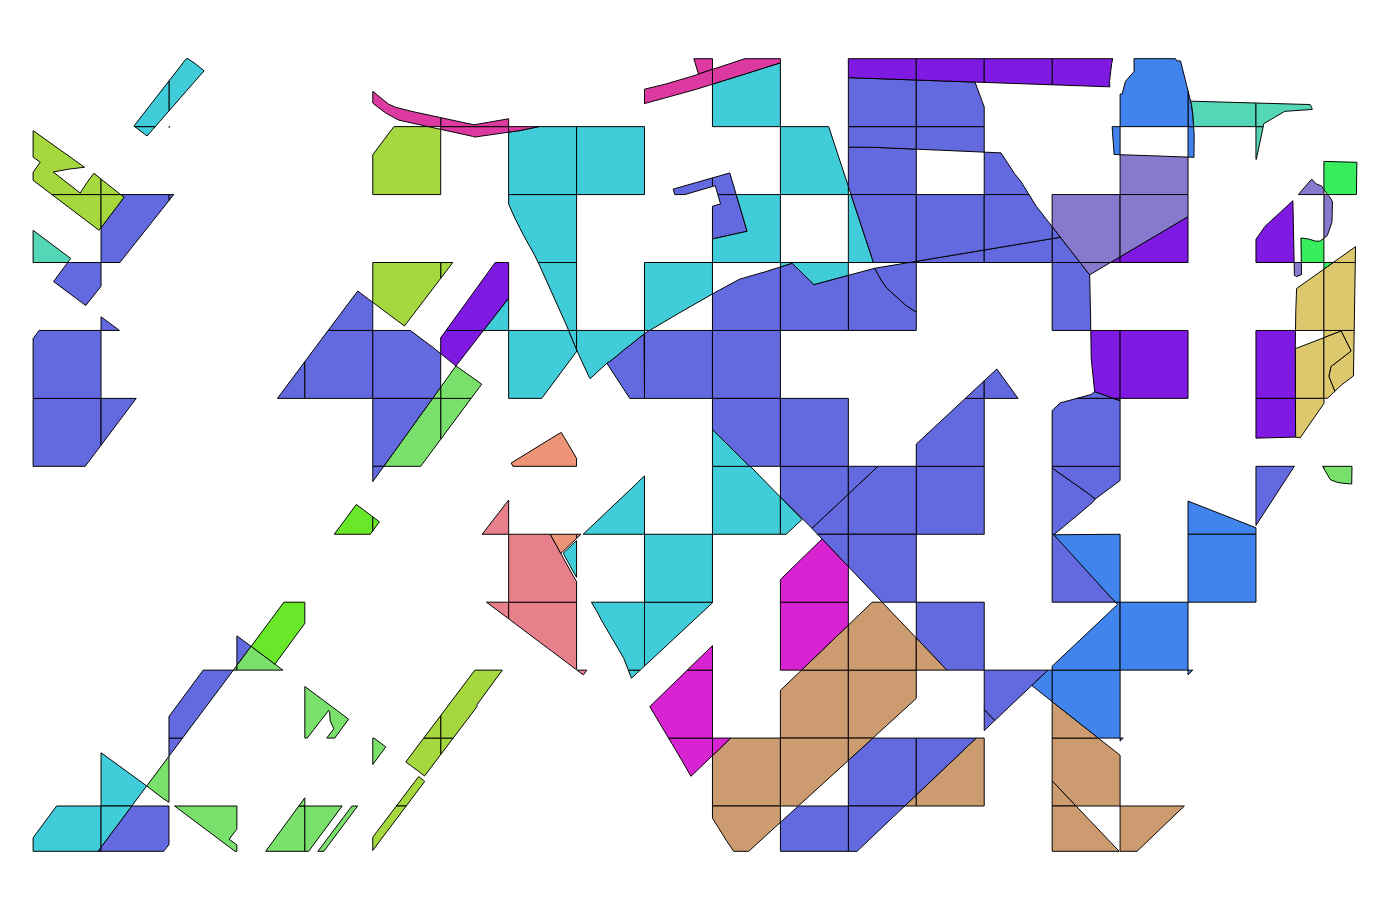
\includegraphics[width=0.7\columnwidth]{Fig/aisa_gt_train.png} \\
            {\bfseries{(a)}} \\
            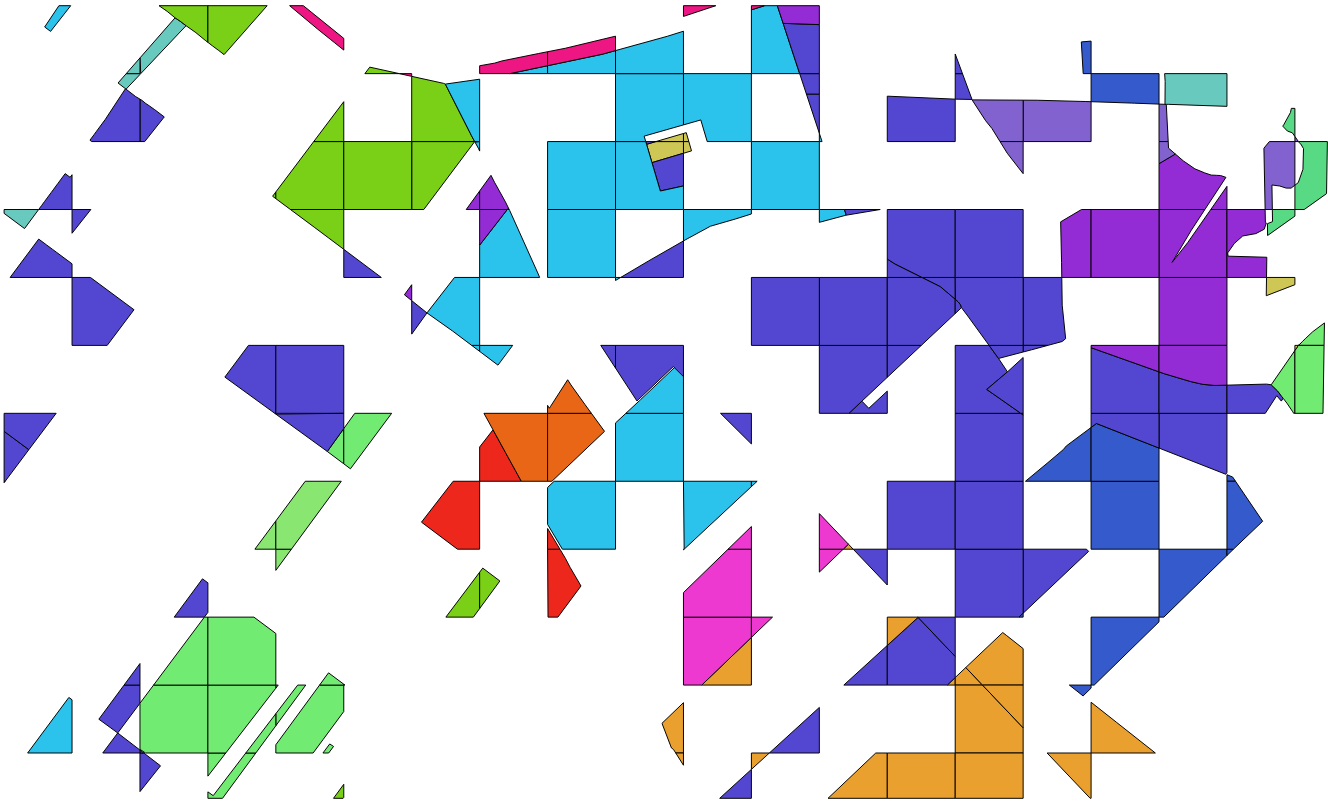
\includegraphics[width=0.7\columnwidth]{Fig/aisa_gt_test.png} \\
            {\bfseries{(b)}} \\
        \end{tabular}
        \caption{Aisa dataset: {\bfseries{(a)}} training polygons of first trial, {\bfseries{(b)}} test polygons of first trial.\label{fig:set-aisa}}
    \end{figure}

    \begin{table}[!t]
        \centering
        \caption{Results of classification with sampling on separate polygons and 20 trials (standard deviation in parenthesis).\label{tab:aisa-otbsimu}}
        \begin{tabular}{|l|c|c|c|}\hline
             & \multicolumn{3}{c|}{\bfseries Cohen's kappa} \\ \hline
            \# samples by class & 250 & 500 & 1000 \\ \hline

            GMM SFS kappa & 0.684 (0.025) & 0.698 (0.027) & 0.711 (0.028) \\
            GMM SFS JM &    0.680 (0.028) & 0.700 (0.028) & 0.710 (0.030) \\
            GMM SFFS JM &   0.680 (0.028) & 0.700 (0.028) & 0.710 (0.030) \\
            GMM ridge &     0.611 (0.040) & 0.620 (0.036) & 0.642 (0.034) \\
            KNN &           0.551 (0.035) & 0.563 (0.033) & 0.574 (0.030) \\
            Random Forest & 0.645 (0.026) & 0.673 (0.023) & 0.693 (0.023) \\

            \hline
        \end{tabular}
    \end{table}

    \begin{table}[!t]
        \centering
        \caption{Mean processing time for training and classification for results of Table \ref{tab:aisa-otbsimu}.\label{tab:aisa-otbsimu-time}}
        \begin{tabularx}{\columnwidth}{|l|*{6}{>{\centering\arraybackslash}X|}}
            \hline
             & \multicolumn{3}{c|}{\bfseries Training time (s)} & \multicolumn{3}{c|}{\bfseries Classification time (s)} \\ \hline
            \# samples by class & 250 & 500 & 1000 & 250 & 500 & 1000 \\ \hline

            GMM SFS kappa & 257 & 496 & 955 & 7.7 & 8.6 & 8.7 \\
            GMM SFS JM &    8.6 & 8.9 & 9.1 & 9.7 & 9.8 & 9.6 \\
            GMM SFFS JM &   8.8 & 9.0 & 9.3 & 9.7 & 9.8 & 9.8 \\
            GMM ridge &     71.7 & 105 & 167 & 530 & 530 & 530 \\
            KNN &           8.9 & 19.6 & 59.7 & 387 & 639 & 887 \\
            Random Forest & 24.5 & 49.3 & 105 & 33.0 & 41.7 & 45.9 \\

            \hline
        \end{tabularx}
    \end{table}

    The results show that, on this dataset, GMM classifiers with selection get the best classification rate. Especially with very few training samples, GMM classifiers with selection seems to outperform the others. In term of computational time, the GMM classifiers are as expected very fast for classification and also for training if the criterion function is not a classification rate. The computation of the kappa seems to suffer from a lack of parallelization which could be improved. Among the three variations of the selection algorithm, none appears to perform better than the others. Using kappa or Jeffries-Matusita distance as criterion is equal and using SFFS does not give any advantage. In this case, using J-M distance as criterion and SFS as search strategy is the best choice in term of time efficiency.

    Nevertheless, good performance are also obtained with Random Forest which becomes more competitive when the number of samples increases.
    The KNN classifier and the GMM classifier with ridge regularization are totally outperform both in term of classification rate and of processing time.

    \subsection{Potsdam dataset}

    This second dataset is built from a dataset of remote sensing images distributed by the International Society for Photogrammetry and Remote Sensing (ISPRS)\footnote{\url{http://www2.isprs.org/commissions/comm3/wg4/2d-sem-label-potsdam.html}}. The dataset is composed of aerial images of the urban area of Potsdam. The area is cut into 38 patches of 6000x6000 pixels with a resolution of 5cm by pixel and 4 channels are available: Red, Blue, Green and Infrared (RGBIR). A Digital Surface Model with same resolution is also provided and a so-called normalized DSM representing the height above ground. The groundtruth for 24 tiles are provided with 6 classes: Low vegetation, High vegetation, Impervious surfaces, Buildings, Cars, Clutter. Table~\ref{tab:potsdam} summarizes the number of samples of each class in the two images used during experimentations. Figure~\ref{fig:potsdam-dataset} shows the complete area and Figure~\ref{fig:potsdam-expl} a particular patch.

    \begin{figure}[!t]
        \centering
        \includegraphics[width=0.7\columnwidth]{Fig/potsdam_full.png}
        \caption{Full Potsdam dataset.\label{fig:potsdam-dataset}}
    \end{figure}

    \begin{figure}[!t]
        \centering
        \includegraphics[width=0.8\columnwidth]{Fig/potsdam_imgexpl.png}
        \caption{Example of patch with {\bfseries{(a)}} orthophoto, {\bfseries{(b)}} DSM and {\bfseries{(c)}} groundtruth.\label{fig:potsdam-expl}}
    \end{figure}

    \begin{table}[!t]
        \centering
        \caption{Repartition of classes in Aisa dataset.\label{tab:potsdam}}
        \begin{tabular}[b]{lrr}\hline
          Class & Number of samples & Number of samples \\
                & in 5\_11          & in 5\_12 \\
          \hline
          Clutter             & 1,078,611  & 812,038 \\
          Trees               & 4,493,295  & 2,132,368 \\
          Cars                & 900,076    & 1,101,541 \\
          Buildings           & 13,469,575 & 17,501,421 \\
          Low vegetation      & 4,718,219  & 3,210,596 \\
          Impervious surfaces & 11,340,224 & 11,242,036 \\
          \hline
        \end{tabular}
    \end{table}

    In the experiment, the following features are computed using the RGBIR images similar to \cite{tuia2015multiclass}:
    \begin{itemize}
        \item Radiometric indexes: NDVI, TNDVI, RVI, SAVI, TSAVI, MSAVI, MSAVI2, GEMI, IPVI, NDWI2, NDTI, RI, CI, BI, BI2 (15 features) \footnote{\url{https://www.orfeo-toolbox.org//Applications/RadiometricIndices.html}};
        \item Morphological profile with reconstruction of each band with a disk of radius 5, 9, 13, 17, 21, 25, 29, 33, 37 and 41 (80 features)\cite{tuia2015multiclass};
        \item Attribute profile of each band with area as attribute and 1000, 2000, 5000, 10000 and 15000 as thresholds (40 features)\cite{tuia2015multiclass};
        \item Attribute profile of each band with diagonal of bounding box as attribute and 100, 200, 500, 1000 and 20000 as thresholds (40 features)\cite{tuia2015multiclass};
        \item Textural features with neighborhood of 19x19 pixels: mean, standard deviation, range and entropy (16 features)\cite{tuia2015multiclass}.
    \end{itemize}
    The normalized DSM and the raw RGBIR image are added to these 191 features and then then stacked to create a new image with 196 bands. The training is made with tile 5\_11 and test with tile 5\_12. Table~\ref{tab:potsdam-otbsimu} presents the results.

    \begin{table}[!t]
        \centering
        \caption{Results of classification with 1000 samples by class and 5 trials (standard deviation in parenthesis).\label{tab:potsdam-otbsimu}}
        \resizebox{\columnwidth}{!}{%
        \begin{tabular}{|l|c|c|c|c|c|}\hline
             & {\bfseries Kappa of} & {\bfseries Kappa of} & {\bfseries Training} & {\bfseries Classif.} & {\bfseries \# features} \\
             & {\bfseries 5\_11 (train)} & {\bfseries 5\_12 (test)} & {\bfseries time (s)} & {\bfseries time (s)} & {\bfseries to classify} \\ \hline

            GMM SFS kappa & 0.694 (0.002) & 0.669 (0.005) & 400 & 310 & 13.2 \\
            GMM SFS JM &    0.624 (0.028) & 0.631 (0.034) & 2 & 310   & 11 \\
            GMM SFFS JM &   0.624 (0.028) & 0.631 (0.034) & 2.6 & 310   & 11 \\
            GMM ridge &     0.632 (0.007) & 0.592 (0.010) & 10 & 2000 & all \\
            KNN &           0.637 (0.005) & 0.607 (0.005) &  &   & all \\
            Random Forest & 0.729 (0.004) & 0.673 (0.005) & 20 & 840  & all \\

            \hline
        \end{tabular}
        }
    \end{table}

    \begin{table}[!t]
        \centering
        \caption{Results of classification with 50000 samples by class and 5 trials (standard deviation in parenthesis).\label{tab:potsdam-otbsimu-big}}
        \resizebox{\columnwidth}{!}{%
        \begin{tabular}{|l|c|c|c|c|c|}\hline
             & {\bfseries Kappa of} & {\bfseries Kappa of} & {\bfseries Training} & {\bfseries Classif.} & {\bfseries \# features} \\
             & {\bfseries 5\_11 (train)} & {\bfseries 5\_12 (test)} & {\bfseries time (s)} & {\bfseries time (s)} & {\bfseries to classify} \\ \hline

            GMM SFS kappa & 0.713 (0.001) & 0.684 (0.001) & 20000 & 340 & 29 \\
            GMM SFS JM &    0.560 (0.111) & 0.576 (0.104) & 6 & 330 & 10 \\
            GMM SFFS JM &   0.560 (0.111) & 0.576 (0.104) & 6.6 & 340 & 10 \\
            GMM ridge &     0.641 (0.015) & 0.611 (0.026) & 460 & 2000 & all \\
            Random Forest & 0.851 (0.001) & 0.715 (0.001) & 2000 & 2000 & all \\

            \hline
        \end{tabular}
        }
    \end{table}

    In this case, the classification rate of GMM classifiers with Jeffries-Matusita distance as criterion function drops clearly and has a high standard deviation. It could be due to the fact that the Gaussian hypothesis, on which this metric relies a lot, is not enough verified. When the classification rate is directly used as criterion, the classifier manages to select the relevant features. It has to be noticed that with kappa only 30 features are selected on average when with Jeffries-Matusita distance, the maximum number of features is selected almost always (set to 60).

    The KNN classifier and the GMM classifier with ridge regularization are again outperformed even if they get stable results.

    Finally, the Random Forest classifier and the GMM with kappa as criterion are from far the best classifiers. The only difference is in the processing time and also a small difference of classification rate with the training image. Random Forest is faster for the training process while the GMM classifier is faster for classifying.

\section{Conclusion}

An algorithm for the classification of high dimension data as hyperspectral image has been presented. The classifier uses GMM model to select iteratively the most relevant features. Several variation of the algorithms has been explored. Experimentations show that allowing backward step in the selection to discard already selected features do not give significant advantages.

Additionally, from the comparison between all the measures used to rank the features, it has been shown that the Jeffries-Matusita distance can be a fast and accurate solution in some case but suffer from some limitations which remain to be determine. A possible explaination could be that this distance does not perform well when data distribution is not similar to a Gaussian distribution. More investigation is needed to confirm this hypothesis. In any case, it is possible to use directly kappa as criterion function even if it implies a loss of time.

Finally, experiments show that the developed GMM classifier performs at least as best as standard classifiers without features selection in particular Random Forest and even outperforms all of them in term of classification time. The next step would be to compare to other feature selection methods.

The second achievement of this work is the development of an efficient implementation using GMM properties to derive fast update rules of the model. The resulting code is available as a remote module of the Orfeo toolbox on Github and make it possible to process huge quantity of high dimension data.

Finally, an improvement could be made to increase the stability of the selected features. For example, with hyperspectral data, a selection of continuous intervals and not band is a possible solution which has already been explored in \cite{serpico2007extraction}.

The python and C++ code are available freely for download: \url{https://github.com/Laadr/FFFS}, \url{https://github.com/Laadr/otbExternalFastFeaturesSelection}.

% \appendices
% \section{Proof of the First Zonklar Equation}
% Appendix one text goes here.

% \section*{Acknowledgment}

% The authors would like to thank...

\bibliographystyle{IEEEtran}
\bibliography{biblio}

% biography section
%
% If you have an EPS/PDF photo (graphicx package needed) extra braces are
% needed around the contents of the optional argument to biography to prevent
% the LaTeX parser from getting confused when it sees the complicated
% \includegraphics command within an optional argument. (You could create
% your own custom macro containing the \includegraphics command to make things
% simpler here.)
%\begin{IEEEbiography}[{\includegraphics[width=1in,height=1.25in,clip,keepaspectratio]{mshell}}]{Michael Shell}
% or if you just want to reserve a space for a photo:

\begin{IEEEbiography}{Michael Shell}
Biography text here.
\end{IEEEbiography}

% if you will not have a photo at all:
\begin{IEEEbiographynophoto}{John Doe}
Biography text here.
\end{IEEEbiographynophoto}

% insert where needed to balance the two columns on the last page with
% biographies
%\newpage

\end{document}



%\begin{figure}[!t]

% An example of a double column floating figure using two subfigures.
% (The subfig.sty package must be loaded for this to work.)
% The subfigure \label commands are set within each subfloat command,
% and the \label for the overall figure must come after \caption.
% \hfil is used as a separator to get equal spacing.
% Watch out that the combined width of all the subfigures on a
% line do not exceed the text width or a line break will occur.
%
%\begin{figure*}[!t]
%\centering
%\subfloat[Case I]{\includegraphics[width=2.5in]{box}%
%\label{fig_first_case}}
%\hfil
%\subfloat[Case II]{\includegraphics[width=2.5in]{box}%
%\label{fig_second_case}}
%\caption{Simulation results for the network.}
%\label{fig_sim}
%\end{figure*}
%
% Note that often IEEE papers with subfigures do not employ subfigure
% captions (using the optional argument to \subfloat[]), but instead will
% reference/describe all of them (a), (b), etc., within the main caption.
% Be aware that for subfig.sty to generate the (a), (b), etc., subfigure
% labels, the optional argument to \subfloat must be present. If a
% subcaption is not desired, just leave its contents blank,
% e.g., \subfloat[].


% An example of a floating table. Note that, for IEEE style tables, the
% \caption command should come BEFORE the table and, given that table
% captions serve much like titles, are usually capitalized except for words
% such as a, an, and, as, at, but, by, for, in, nor, of, on, or, the, to
% and up, which are usually not capitalized unless they are the first or
% last word of the caption. Table text will default to \footnotesize as
% the IEEE normally uses this smaller font for tables.
% The \label must come after \caption as always.
%
%\begin{table}[!t]
%% increase table row spacing, adjust to taste
%\renewcommand{\arraystretch}{1.3}
% if using array.sty, it might be a good idea to tweak the value of
% \extrarowheight as needed to properly center the text within the cells
%\caption{An Example of a Table}
%\label{table_example}
%\centering
%% Some packages, such as MDW tools, offer better commands for making tables
%% than the plain LaTeX2e tabular which is used here.
%\begin{tabular}{|c||c|}
%\hline
%One & Two\\
%\hline
%Three & Four\\
%\hline
%\end{tabular}
%\end{table}


% Note that the IEEE does not put floats in the very first column
% - or typically anywhere on the first page for that matter. Also,
% in-text middle ("here") positioning is typically not used, but it
% is allowed and encouraged for Computer Society conferences (but
% not Computer Society journals). Most IEEE journals/conferences use
% top floats exclusively.
% Note that, LaTeX2e, unlike IEEE journals/conferences, places
% footnotes above bottom floats. This can be corrected via the
% \fnbelowfloat command of the stfloats package.